\label{chapter:background}

In this chapter we discuss the background on which our work is based. We first present text summarization and outline the different levels on which this can be done (Section \ref{sec:summarization}). We then introduce the notion of \textit{syntactic parsing}, which respectively allows us to understand the grammatical structure of a sentence as well as the relations between its constituents (Section \ref{sec:syntactic_parsing}). Then, we explain a number of logic programming concepts which will later be necessary for the description of our implementation (Section \ref{sec:asg}). Finally, we give a brief overview of the Machine Learning concepts we make use of in order to evaluate our system (Section \ref{sec:neural_networks}).

\section{Summarization}
\label{sec:summarization}

Summarization is a general task which consists of taking the most important information from a passage and rewriting it into a more concise form, using at most half the amount of text \cite{lloret_text_2008}.

\subsection{Types Of Summaries}

In what follows we discuss different ways in which we can characterise summaries. Firstly, summaries can be grouped into one of the two following categories, depending on how they are built:

\begin{itemize}
\item An \textit{extractive} summary is made up of chunks of sentences which are copied word-for-word from the original text.
\item An \textit{abstractive} summary is a rewriting of the text's content in a more concise form.
\end{itemize}

\noindent
Summaries can focus on different sections or topics of the text, allowing us to differentiate between the two following types:

\begin{itemize}
\item \textit{Generic} summaries do not try and focus on anything in particular, they simply aim to recount the most important features.
\item \textit{Focused} (or \textit{query-driven}) summaries, on the other hand, require a user-input, which specifies the focus of the summary.
\end{itemize}

\noindent
We can also differentiate the purpose of summaries \cite{radev_introduction_2002} (see example in Figure \ref{fig:indicative_informative_summaries}):

\begin{itemize}
\item \textit{Indicative} summaries aim to outline what a text is about, without going into much detail.
\item \textit{Informative} summaries, on the other hand, take the content from an original document and give a shortened version of it.
\end{itemize}

\begin{figure}[H]
\begin{subfigure}{\textwidth}
\begin{displayquote}
Yellow warnings of strong winds were put in place for parts of the UK. These very strong winds are likely to cause travel disruption, so those in affected areas are advised to take extra care when driving on exposed routes. In addition, heavy rain is expected in parts of the country, which could cause local flooding.
\end{displayquote}
\caption{\textit{Indicative} summary}
\vspace{\baselineskip}
\end{subfigure}
\begin{subfigure}{\textwidth}
\begin{displayquote}
It’s going to be windy across the western half of the UK, with gusts reaching 60 to 70mph along Irish Sea coastlines, the west of Scotland and perhaps some English Channel coasts. Those in affected areas are advised to take extra care when driving on bridges or high open roads. Flood warnings were issued on Sunday for two areas – Keswick campsite in Cumbria and a stretch along the River Nene east of Peterborough.
\end{displayquote}
\caption{\textit{Informative} summary}
\end{subfigure}
\caption[]{Example of \textit{indicative} and \textit{informative} summaries for a news article\footnotemark}
\label{fig:indicative_informative_summaries}
\end{figure}

\footnotetext{Article from The Guardian about storm Brendan: \url{https://www.theguardian.com/uk-news/2020/jan/12/storm-brendan-gales-forecast-uk}}

\subsection{Summarization Levels}

Depending on the level of detail at which text analysis is done, we identify three different levels of summarization \cite{lloret_text_2008}: \textit{surface}, \textit{entity} and \textit{discourse}. Many current systems employ what is called a \textit{hybrid} approach, combining techniques from different summarization levels.

\subsubsection*{Surface Level}

On a \textit{surface level}, little text analysis is performed, and we rely on keywords in the text which are later combined to generate a summary. Techniques which are common include:

\begin{itemize}
\item \textit{Thematic features} are identified by looking at the words that appear most frequently. Usually, the sentences in a passage containing the most important information have a higher probability of containing these \textit{thematic features}.
\item Often, the \textit{location} of a sentence can help identify its importance; the first and last sentences are generally a good indicator for the respective introduction and conclusion of a document. Moreover, we may use the title and heading (if any) to find out which topics are most relevant.
\item \textit{Cue words} are expressions like ``in this article" and ``to sum up"; these can give us a clue as to where the relevant information is.
\end{itemize}

\subsubsection*{Entity Level}

A more analytic approach can be done at an \textit{entity level}, where we build a model of a document's individual entities (i.e., words or phrases) and see how they relate. Common techniques are:

\begin{itemize}
\item \textit{Similarity} between different words or groups of words, whether it be synonyms or terms relating to the same topic.
\item \textit{Logical relations} involve the use of a connector such as ``before" or ``therefore", and tell us how the information given by such connected phrases relates.
\end{itemize}

\subsubsection*{Discourse Level}

Finally at a \textit{discourse level} we go beyond the contents of a text, exploiting its structure instead. Some of the things we can analyse are:

\begin{itemize}
\item The \textit{format} can be taken into account to help us extract key information. For example, in a rich-text document we may want to pay close attention to terms that are underlined or italicized.
\item The \textit{rhetorical structure} can tell us whether the document is argumentative or narrative in nature. In the latter case a more concise description of the text's contents would suffice, while the former would involve recounting the key points and conclusions made by the author.
\end{itemize}

\section{Syntactic Parsing}
\label{sec:syntactic_parsing}

\textit{Tokenization} is the processes of splitting a text into its individual \textit{tokens}, or words. To each of these \textit{tokens} we can assign a position of speech (POS) tag, which tells us what type of word this is (see Appendix \ref{appendix:pos}). Additionally, each of these \textit{tokens} is assigned a \textit{lemma}, which is essentially the ``neutral" form of a word, be it the singular of a noun or the base form of a verb.

Furthermore, \textit{syntactic parsing} is a technique that reveals the grammatical links between POS tagged \textit{tokens} \cite{noauthor_syntactic_nodate}, the result of which can then be visualised in what is called a \textit{parse tree}. This type of \textit{syntactic parsing} is known as \textit{constituency parsing}. An example of such a \textit{parse tree} is shown in Figure \ref{fig:constituency_tree_basic_sentence} for one of the first of the two most prominent \textit{syntactic parsers}: \textbf{CoreNLP}\footnote{CoreNLP is an NLP toolkit developed by Stanford: \url{https://corenlp.run}} and \textbf{spaCy}\footnote{spaCy is an NLP toolkit that integrates with deep learning libraries: \url{https://spacy.io}}.

\begin{figure}[H]
\centering
\begin{tabular}{c}
\begin{lstlisting}[numbers=none, basicstyle=\ttfamily, columns=fixed]
                   S                          
             ______|________________________   
            NP                VP            | 
         ___|______        ___|______       |  
        NP         |      |         ADJP    | 
   _____|___       |      |          |      |  
 NNP       POS     NN    VBZ         JJ     . 
  |         |      |      |          |      |  
Albert      's chocolate  is     delicious  .
\end{lstlisting}
\end{tabular}
\caption{\textit{Constituency parse tree} for a basic sentence, as generated by  \textbf{CoreNLP}}
\label{fig:constituency_tree_basic_sentence}
\end{figure}

\noindent
Moreover, many \textit{syntactic parsers} are also capable of \textit{dependency parsing}, which involves linking the \textit{tokens} in a sentence using binary asymmetric relations called \textit{dependencies} \cite{kubler_dependency_nodate}. These \textit{dependencies} can help us understand the connections between different \textit{tokens} when visualised in the form of a \textit{parse tree}, as illustrated in Figure \ref{fig:dependency_tree_basic_sentence}.

\begin{figure}[H]
\centering
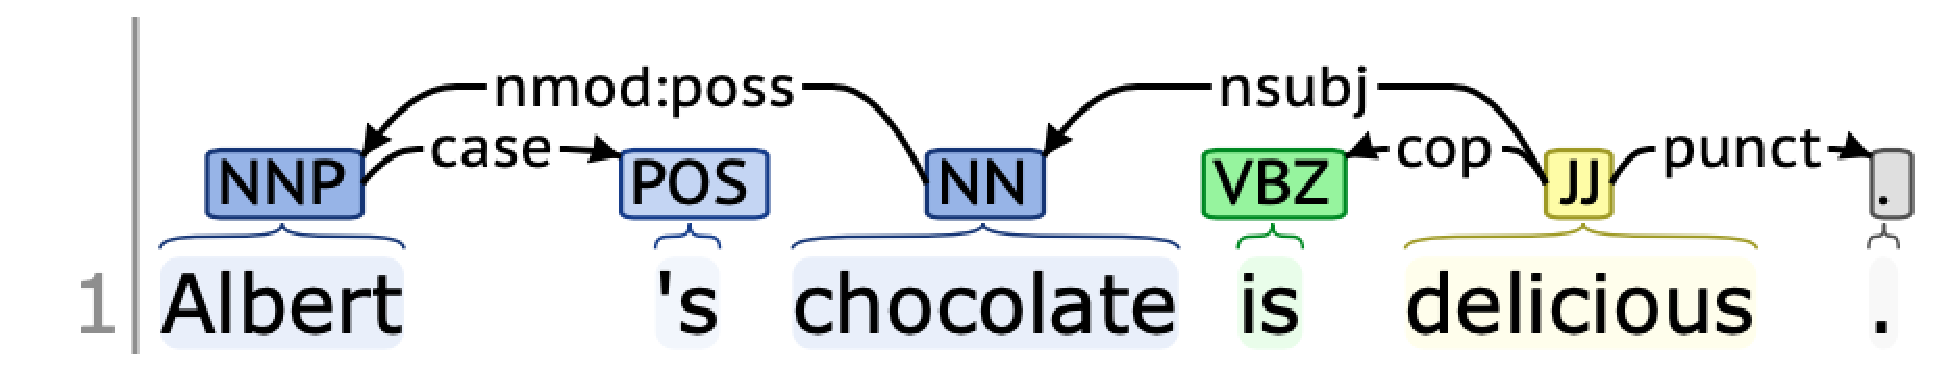
\includegraphics[width=0.75\textwidth]{basic_sentence_core_nlp.eps}
\caption{\textit{Dependency tree} for a basic sentence, as generated by  \textbf{CoreNLP}}
\label{fig:dependency_tree_basic_sentence}
\end{figure}

\noindent
However, the English language can often be ambiguous and highly context-dependent, meaning that multiple interpretations may be possible, resulting in different \textit{parse trees} for the same sentence. Consider the following two sentences \cite{noauthor_studying_nodate}:

\begin{displayquote}
He fed her cat food. \\
I saw a man on a hill with a telescope.
\end{displayquote}

\noindent
Depending on the context, we could interpret the first sentence as a person who either fed a woman's cat, fed a woman some cat food, or fed the cat food itself. Although the last meaning does not make much sense, this is one that \textbf{CoreNLP} chooses, as shown in Figure \ref{fig:dependency_tree_ambiguous_sentence}. Therefore, it very important to first accurately perform \textit{syntactic parsing} if we then want to produce a summary which is coherent with the original text \cite{gomez-rodriguez_how_2019}.

\begin{figure}[H]
\centering
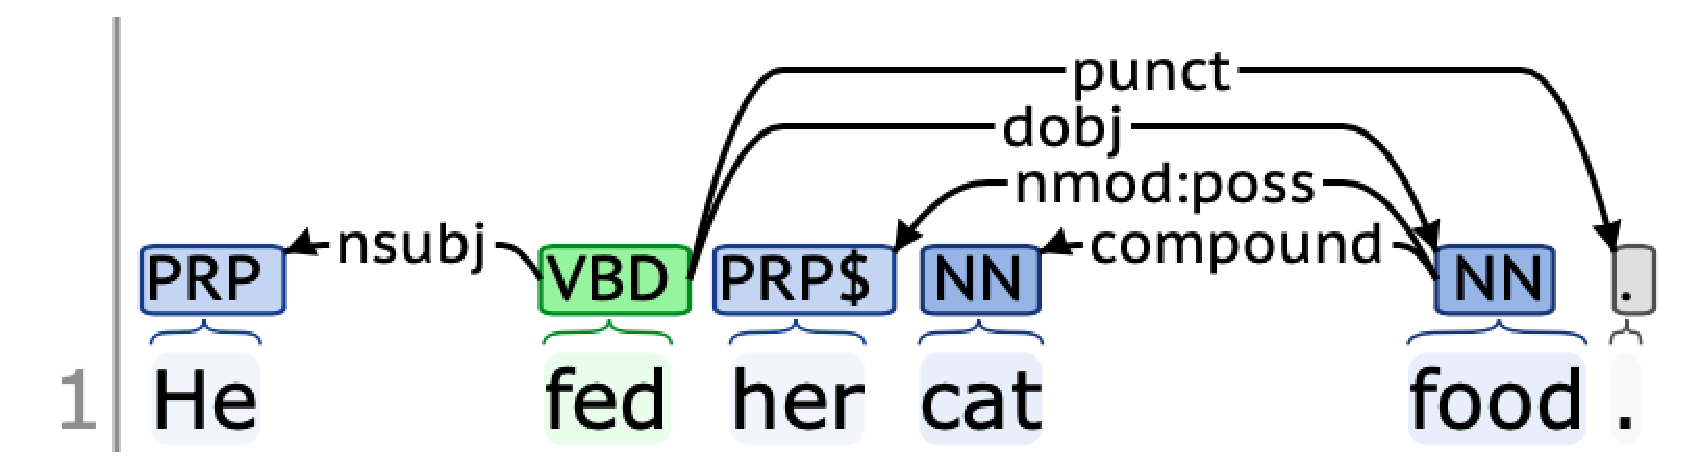
\includegraphics[width=0.75\textwidth]{ambiguous_sentence_core_nlp.eps}
\caption{\textit{Constituency tree} for an ambiguous sentence, as generated by  \textbf{CoreNLP}: here, ``cat food" is interpreted as a compound entity belonging to ``her", erroneously meaning that a man fed a woman's ``cat food"}
\label{fig:dependency_tree_ambiguous_sentence}
\end{figure}

\section{Answer Set Grammars}
\label{sec:asg}

Logic programming is a programming paradigm based on formal mathematical logic. It was introduced by R. Kowalski in 1974 and is highly suitable for knowledge representation \cite{apt_logic_1990}. Since its introduction, it provided inspiration for a number of languages, such as Answer set programming (ASP).

\subsection{Answer Set Programming}

ASP is a declarative first-order (predicate) logic language whose aim is to solve complex search problems \cite{lifschitz_what_nodate}. When asked to solve a problem ASP returns a list of \textit{answer sets} (or \textit{stable models}), whose definition (see Definition \ref{def:answer_set}) we will give after having introduced a number of concepts pertinent to logic programming.

\begin{definition}[Term \cite{kowalski_predicate_1974}]
A \textit{term} is either a \textit{variable} $x,y,z,...$ or an expression $f(t_1,t_2,...,t_k)$, where $f$ is a k-ary \textit{function symbol} and the $t_i$ are \textit{terms}. A \textit{constant} is a 0-ary \textit{function symbol}.
\end{definition}

\begin{definition}[Atom \cite{kowalski_predicate_1974}]
An \textit{atomic formula} (or \textit{atom}) has the form $P(t_1,t_2,...,t_k)$, where $P$ is a k-ary predicate (boolean function) symbol and the $t_i$ are terms.
\end{definition}

\noindent
In ASP, a \textit{literal} is an \textit{atom} \textit{a} or its negation \textit{not a} (we call this ``negation as failure"). ASP programs are composed of a set of \textit{normal rules} whose head is a single \textit{atom} and whose body is a conjunction of \textit{literals} \cite{law_representing_2019}.

\begin{equation}
\underbrace{h}_{\textit{head}} \leftarrow \underbrace{b_1, b_2, ..., b_k, \text{not}\ b_{k+1}, ..., \text{not}\ b_m}_{\textit{body}}.
\end{equation}

\noindent
If the body is empty ($k = m = 0$) then a rule is called a \textit{fact}. We can also have \textit{constraints}, which are like \textit{normal rules} except that the head is empty. These prevent any \textit{answer sets} from both including $b_1, b_2, ..., b_k$ and excluding $b_{k+1}, ..., b_m$.

To compute the \textit{reduct} of a program (see Definition \ref{def:reduct}), we are first going to need to understand the notion of \textit{Herbrand base}. The \textit{Herbrand base} of a program P, denoted $HB_P$, is the set of variable-free (\textit{ground}) \textit{atoms} that can be formed from predicates and \textit{constants} in P. The subsets of $HB_P$ are called the (Herbrand) \textit{interpretations} of P \cite{law_representing_2019}.

\begin{definition}[Reduct \cite{law_representing_2019}]
\label{def:reduct}
Given a program P and a \textit{Herbrand interpretation} $I \subseteq HB_P$, the \textit{reduct} $P^I$ is constructed from the grounding of P in three steps:
\begin{enumerate}[nolistsep]
\item Remove rules whose bodies contain the negation of an atom in I.
\item Remove all negative \textit{literals} from the remaining rules.
\item Replace the head of any constraint with $\bot$ (where $\bot \notin HB_P$).
\end{enumerate}
For example, the \textit{reduct} of the program $\{a \leftarrow \text{not}\ b, c.\quad d \leftarrow \text{not}\ c.\}$ with respect to $I=\{b\}$ is $\{d.\}$.
\end{definition}

\noindent
Given a set $A$, a \textit{ground normal rule} of P is \textit{satisfied} if the head is in $A$ when all positive \textit{atoms} and none of the negated \textit{atoms} of the body are in $A$; that is, when the body is \textit{satisfied}. A \textit{ground constraint} is \textit{satisfied} when its body is not \cite{law_representing_2019}.

\begin{definition}[Minimal Model]
We say that $I$ is a (Herbrand) \textit{model} when $I$ \textit{satisfies} all the rules in the program P. It is a \textit{minimal model} if there exists no smaller \textit{model} than $I$.
\end{definition}

\begin{definition}[Answer Set \cite{law_representing_2019}]
\label{def:answer_set}
Any $I \subseteq HB_P$ is an \textit{answer set} of P if it is equal to the \textit{minimal model}  of the \textit{reduct} $P^I$. We will denote the set of \textit{answer sets} of a program P with $AS(P)$. 
\end{definition}

\subsection{Answer Set Grammars}

A context-free grammar (CFG) is a grammar characterised by a set of \textit{production rules} that describe all possible strings which can be formed by this grammar. Before discussing ASGs though we must first formally define CFGs (see Definition \ref{def:cfg}), and introduce the notion of a \textit{parse tree} in the current context (see Definition \ref{def:parse_tree}).

\begin{definition}[Context-Free Grammar \cite{scheinberg_note_1960}]
\label{def:cfg}
A CFG is a finite set G of \textit{production rules} $\alpha \to \beta$, where $\alpha$ is a single symbol and $\beta$ is a finite string of symbols from a finite alphabet (vocabulary) V. V contains precisely the symbols appearing in these rules plus the ``boundary" symbol $\epsilon$, which does not appear in these rules. Rules of the form $\alpha \to \alpha$ (which have no effect) are not allowed.
\end{definition}

\begin{definition}[Parse Tree \cite{law_representing_2019}]
\label{def:parse_tree}
Let $G_{CF}$ be a CFG. A \textit{parse tree} $PT$ of $G_{CF}$ for a given string consists of a node $node(PT)$, a list of \textit{parse trees}, called \textit{children} and denoted $children(PT)$, and a rule $rule(PT)$, such that:
\begin{enumerate}[nolistsep]
\item If $node(PT)$ is a terminal node, then $children(PT)$ is empty.
\item If $node(PT)$ is non-terminal, then $rule(PT)$ is of the form $node(PT) \to n_1 ... n_k$ where each $n_i$ is equal to the node of the $ith$ element in $children(PT)$, and $|children(PT)| = k$.
\end{enumerate}
\end{definition}

\begin{definition}[Trace \cite{law_representing_2019}]
We can represent each node n in a \textit{parse tree} by its \textit{trace}, $trace(n)$, through the tree. The \textit{trace} of the root is the empty list \texttt{[]}; the i\textsuperscript{th} child of the root is \texttt{[i]}; the j\textsuperscript{th} child of the i\textsuperscript{th} child of the root is \texttt{[i, j]}, and so on.
\end{definition}

\noindent
These concepts are illustrated in Figure \ref{fig:cfg_parse_tree_example}, where we have written a set of \textit{production rules} for the grammar \texttt{a\textsuperscript{i}b} (i.e., strings consisting of any number of ``a"s followed by a ``b"), along with a \textit{parse tree} for the specific string ``aab".

\begin{figure}[H]
\begin{subfigure}{0.3\textwidth}
\texttt{1: start -> as "b" \\ 2: as -> "a" as \\ 3: as ->\\}
\caption{CFG for \texttt{a\textsuperscript{i}b}}
\end{subfigure}
\begin{subfigure}{0.34\textwidth}
\begin{table}[H]
\centering
\begin{tabular}{@{}ccc@{}}
\toprule
\textbf{$trace(n)$} & \textbf{$node(n)$} \\ \midrule
\texttt{[]} & \texttt{start} \\
\texttt{[1]} & \texttt{as} \\
\texttt{[1,1]} & \texttt{a} \\
\texttt{[1,2]} & \texttt{as} \\
\texttt{[1,2,1]} & \texttt{a} \\
\texttt{[1,2,2]} & \texttt{as} \\
\texttt{[2]} & \texttt{b} \\ \bottomrule
\end{tabular}
\end{table}
\caption{\textit{Parse tree} table for \texttt{aab}}
\end{subfigure}
\begin{subfigure}{0.34\textwidth}
\centering
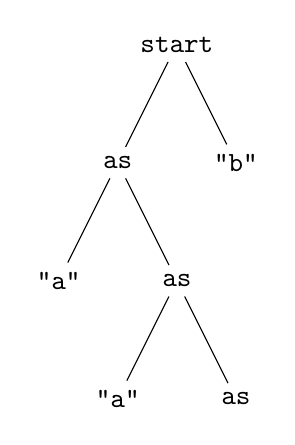
\begin{tikzpicture}
\node {\texttt{start}}
  child {node {\texttt{as}}
    child {node {\texttt{"a"}}}
    child {node {\texttt{as}}
      child {node {\texttt{"a"}}}
      child {node {\texttt{as}}}}}
  child {node {\texttt{"b"}}};
\end{tikzpicture}
\caption{\textit{Parse tree} graph for \texttt{aab}}
\end{subfigure}
\caption{Example of a CFG for the grammar \texttt{a\textsuperscript{i}b}}
\label{fig:cfg_parse_tree_example}
\end{figure}

\noindent
ASGs are an extension of CFGs, whereby each \textit{production rule} is \textit{annotated} (see Definition \ref{def:annotated_production_rule}). Using these \textit{annotated production rules}, it is possible to vastly reduce the complexity of the structures that can be produced by a grammar.

\begin{definition}[Annotated ASP Program \cite{law_representing_2019}]
An \textit{annotated} ASP program is an ASP program where some atoms are annotated with a \textit{ground} term. For instance, the \textit{annotated} \textit{atom} a(1)@2 represents the \textit{atom} a(1) with the annotation 2.
\end{definition}

\begin{definition}[Annotated Production Rule \cite{law_representing_2019}]
\label{def:annotated_production_rule}
An \textit{annotated production rule} is of the form $n_0 \to n_1 ... n_k\ P$ where $n_0 \to n_1 ... n_k$ is an ordinary CFG \textit{production rule} and $P$ is an \textit{annotated} ASP program, with every \textit{annotation} being an integer from $1$ to $k$.
\end{definition}

\noindent
In the context of ASGs, the annotations in each \textit{annotated} ASP program refer to index of a node's child. For instance, \texttt{a(1)@2} can be read as the truth value of the \textit{term} \texttt{a(1)} in the \textit{annotated} ASP program of the second child of the node whose \textit{production rule} we are in.

An example is shown in Figure \ref{fig:asg_example}, where we have written \textit{annotated production rules} for the language \texttt{a\textsuperscript{n}b} ($\texttt{n} \ge 2$). By restricting this grammar to strings which contain at least two ``a"s, we have effectively captured a subset of the language shown in Figure \ref{fig:cfg_parse_tree_example}.

\begin{figure}[H]
\centering
\begin{tabular}{c}
\begin{lstlisting}[numbers=none, basicstyle=\ttfamily, columns=fixed, basewidth=0.45em]
1: start -> as "b" { :- size(X)@1, X < 1. }
2: as -> "a" as    { size(X+1) :- size(X)@2. }
3: as ->           { size(0). }
\end{lstlisting}
\end{tabular}
\\ \leavevmode \\ * Intuitively, \texttt{size} represents the length of the current string.
\caption{Example of an ASG for the grammar \texttt{a\textsuperscript{n}b}, where $\texttt{n} \ge 2$}
\label{fig:asg_example}
\end{figure}

\noindent
In order to understand the notion of \textit{satisfiability} for a given \textit{parse tree} with respect to an \textit{annotated} grammar, we must first formally define what is a \textit{conforming parse tree} (see Definition \ref{def:conforming_parse_tree}).

\begin{definition}[Parse Tree Program \cite{law_representing_2019}]
Let G be an ASG and PT be a \textit{parse tree}. $G[PT]$ is the program $\{\ rule(n)@trace(n)\ |\ n \in PT\ \}$, where for any \textit{production rule} $n_0 \to n_1...n_k\ P$, and any trace $t$, $PR@t$ is the program constructed by replacing all annotated atoms $a@i$ with the atom $a@t++[i]$ and all \textit{unannotated atoms} $a$ with the atom $a@t$ ($++$ being the concatenation operator).
\end{definition}

\begin{definition}[Conforming Parse Tree \cite{law_representing_2019}]
\label{def:conforming_parse_tree}
Given a string $str$ of terminal nodes, we say that $str \in \mathcal{L}(G)$ ($str$ \textit{conforms} to the language of G) if and only if there exists a parse tree PT of G for $str$ such that the program $G[PT]$ is \textit{satisfiable}. For such a PT, every single rule in the language must be \textit{satisfied}.
\end{definition}

\noindent
The \textit{parse tree program} $G[PT]$ corresponding to the \textit{annotated production rules} shown in Figure \ref{fig:asg_example} is given in Figure \ref{fig:asg_tree_program_example}. This program has a single \textit{answer set} $\{size(0)@[1,2,2],\ size(1)@[1,2],\ size(2)@[1]\}$. From this example, it is easy to see how the corresponding program would be \textit{unsatisfiable} for the string \texttt{ab}.

\begin{figure}[H]
\centering
\texttt{:- size(X)@[1], X < 1. \\
           size(X+1)@[1] :- size(X)@[1,2]. \\
           size(X+1)@[1,2] :- size(X)@[1,2,2]. \\
           size(0)@[1,2,2].}
\caption{$G[PT]$ for the \textit{parse tree} and ASG from the examples above}
\label{fig:asg_tree_program_example}
\end{figure}

\subsection*{Learning Answer Set Grammars}

Given an incomplete ASG, it is possible to learn the complete grammar by induction (which uses \textbf{ILASP}\footnote{ILASP is a logic-based machine learning system: \url{http://www.ilasp.com}}), as long as we provide some \textit{positive examples} (strings which should conform to the language) and/or \textit{negative examples}  (strings which must not), as well as a \textit{hypothesis space} and usually some \textit{background} information. Note that the \textit{background} is only used for ``global" knowledge, such as defining what is a number, or how to increment one \cite{law_representing_2019}.

In such an \textit{inductive learning program} (ILP) task, we have a \textit{hypothesis space} in the form of \textit{mode declarations}, defining the format of the heads (written \texttt{\#modeh}) and bodies (written \texttt{\#modeb}) of \textit{production rules} which can be learned. It is also possible to restrict the scope of a particular \textit{mode declaration} by specifying a list of rule numbers at the end. Note that there are two forms of body \textit{mode declarations}: \texttt{\#modeba} is used for predicates that accept an $@$ \textit{annotation}, and \texttt{\#modebb} is intended for those without (which are defined in \texttt{\#background}). An example is shown in Figure \ref{fig:asg_ilp_example}.

\begin{figure}[H]
\centering
\begin{subfigure}{0.55\textwidth}
\texttt{start -> as bs \{\} \\
as -> "a" as \{\} | \{\} \\
bs -> "b" bs \{\} | \{\} \\
\newline
+ [] \\
+ ["a", "b"] \\
+ ["a", "a", "b", "b"] \\
- ["a"] \\
- ["b"] \\
- ["a", "a"] \\
- ["b", "b"] \\
- ["a", "a", "b"] \\
- ["a", "b", "b"] \\
\newline
\#background \{ \\
num(0). num(1). num(2). num(3). \\
inc(X,X+1) :- num(X), num(X+1). \} \\
\newline
\#modeh(size(var(num))):[2,3,4,5]. \\
\#modeh(size(0)):[2,3,4,5]. \\
\#modeba(size(var(num))). \\}
\caption{Input incomplete program}
\end{subfigure}
\begin{subfigure}{0.44\textwidth}
\texttt{start -> as bs \{ \\
\phantom{ }:- not size(X)@2, size(X)@1. \\
\} \\
\newline
as -> "a" as \{ \\
\phantom{ }size(X+1) :- size(X)@2. \\
\} \\
\newline
as -> \{ \\
\phantom{ }size(0). \\
\} \\
\newline
bs -> "b" bs \{ \\
\phantom{ }size(X+1) :- size(X)@2. \\
\} \\
\newline
bs -> \{ \\
\phantom{ }size(0). \\
\}} \\
\caption{Output learned program}
\end{subfigure}
\newline
\newline
* Note: the symbol \texttt{|} indicates multiplicity of \textit{production rules}.
\caption{Example of an ASG ILP task for the language \texttt{a\textsuperscript{n}b\textsuperscript{n}}}
\label{fig:asg_ilp_example}
\end{figure}

\section{Neural Networks}
\label{sec:neural_networks}

In this section we present the concepts which will later be necessary to understand the evaluation of our project.

A neural network is a set of \textit{neurons} organized in layers. Each \textit{neuron} can be seen as a placeholder for a numerical value and in between each layer a non linear differentiable function is applied

\subsection{Recurrent Neural Networks}



RNNs address the problem of applying neural networks on sequential data... 
an RNN will hold a internal state vector that it will update at each step....







A recurrent neural network (RNN) is a chain-like neural network that is applied once for each \textit{token} in the input sequence \cite{cho_learning_2014}. At each timestep $t$ in a ``vanilla" RNN (i.e., for each item in the sequence), the current \textit{hidden state} $h_t$ is computed as a function of the previous \textit{hidden state} $h_{t-1}$ and the current input \textit{token} $x_t$, using a non-linear \textit{activation function} (usually sigmoid) \cite{cho_learning_2014}.

\subsection{Long Short-Term Memories}

A long short-term memory (LSTM) is a particular kind of RNN, motivated by the problems of vanishing and exploding gradients which sometimes occur due to the chain-like nature of RNNs. The solution here is to at each timestep use what is called a \textit{memory block}, which holds at it center a linear unit that is connected to itself. In addition, it has three \textit{gates}: input ($i$), forget ($f$) and output ($o$). Respectively, these three \textit{gates} are concerned with which information to store, how long to store it, and when it should be passed on \cite{gers_learning_2000}.

Finally, each \textit{memory block} also stores a \textit{cell state} $c_t$, which combines information from the previous \textit{cell state} $c_{t-1}$ and from the \textit{candidate state} $g_t$ (defined as per the \textit{hidden state} in a vanilla RNN), using the \textit{forget} and \textit{input} \textit{gates} to regulate information flow. The \textit{hidden state} $h_t$ is then defined as a function of this \textit{cell state}, controlled by the \textit{output gate}. Figure \ref{fig:memory_block} shows this diagrammatically \cite{graves_hybrid_2013}.

\begin{equation}
\begin{aligned}
i_t &= \sigma(W_{xi} \cdot x_t + W_{hi} \cdot h_{t-1} + W_{ci} \cdot c_{t-1} + b_i) \\
f_t &= \sigma(W_{xf} \cdot x_t + W_{hf} \cdot h_{t-1} + W_{cf} \cdot c_{t-1} + b_f) \\
o_t &= \sigma(W_{xo} \cdot x_t + W_{ho} \cdot h_{t-1} + W_{co} \cdot c_t + b_o) \\
g_t &= tanh(W_{xg} \cdot x_t + W_{hg} \cdot h_{t-1} + b_g) \\
c_t &= f_t \cdot c_{t-1} + i_t \cdot g_t \\
h_t &= tanh(c_t)
\end{aligned}
\end{equation}

\begin{figure}[H]
\centering
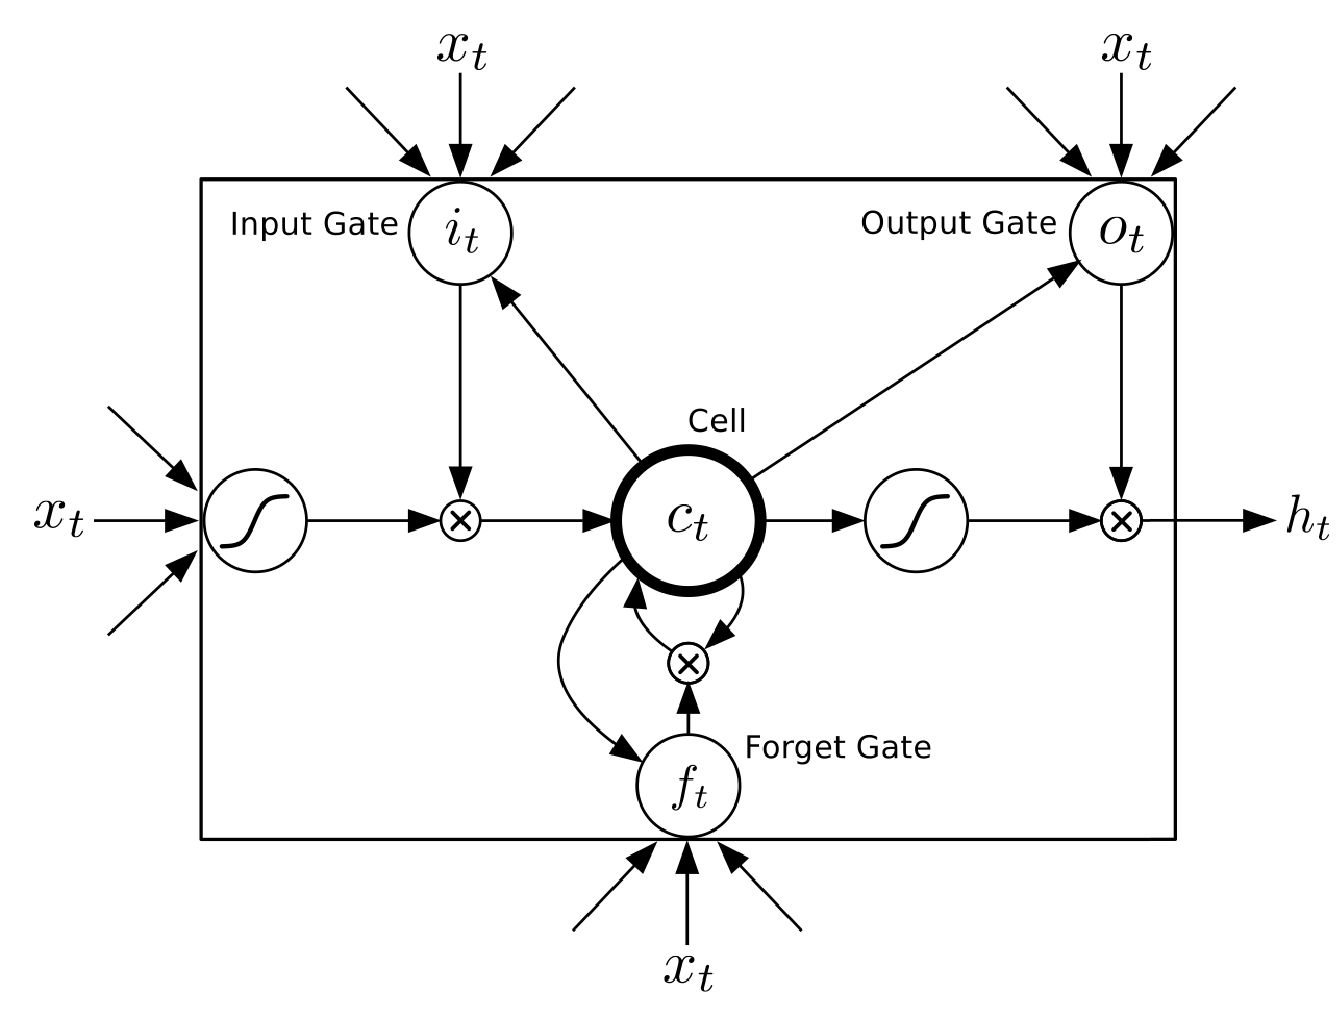
\includegraphics[width=0.62\textwidth]{memory_block.eps}
\caption{\cite{graves_hybrid_2013} Diagram showing the flow of information in an LSTM \textit{memory block}}
\label{fig:memory_block}
\end{figure}

\subsection{Encoder-Decoders}

An \textit{encoder-decoder} is a neural network consisting of two eponymous RNNs, which are often LSTMs. The \textit{encoder}'s job is to translate any variable-length sequence given as input into a fixed-length vector representation, while the \textit{decoder}'s role is to transform this into a new variable-length sequence. Together, they are trained to maximize the probability of generating a target sequence given the corresponding input sequence \cite{cho_learning_2014}.

\subsection{Attention Mechanism}

In the context of neural machine translation (NMT) systems such as \textit{encoder-decoders}, the idea behind \textit{attention} is to improve performance by selectively looking at sub-portions of the input sequence, which becomes especially important for long sequences of text \cite{yao_dual_2018}.

\subsubsection{Global Attention}

On top of being dependant on the last \textit{hidden state} $d_{t-1}$ and output \textit{token} $y_{i-1}$, every \textit{hidden state} $d_t$ in a \textit{decoder} with \textit{global attention} is computed also in function of its \textit{context vector} $c_t$. Each \textit{context vector} $c_t$ is defined as a weighted sum of the \textit{encoder}'s \textit{hidden states} $h_i$. The $h_i$ that are assigned a higher weight are those which are more similar to $d_t$, which is done using a trainable \textit{alignment model} $a$ \cite{bahdanau_neural_2016}.

\begin{equation}
\begin{aligned}
c_t &= \sum_{i} \alpha_{ti} \cdot h_t \\
\mbox{where } \alpha_{ti} &= \frac{exp(s_{ti})}{\sum_{j} exp(s_{tj})} \\
s_{ti} &= a(d_{t-1},h_i)
\end{aligned}
\end{equation}

Here the idea is that $\alpha_{ti}$ tells us how important each $h_i$ is with respect to the current timestep $t$, influencing the value of $d_t$ and hence the decision of the generated output \textit{token} $y_t$. Essentially, this is a way of telling the \textit{decoder} which parts of the input sequence to pay attention to. Thanks to this mechanism, the \textit{encoder} is no longer forced to compress all the useful information from an input sequence into a fixed-length vector, thus improving performance for longer sequences of \textit{tokens} \cite{bahdanau_neural_2016}.